\chapter{Definition of the experimental platform}
\lhead{Chapter 4. \emph{Definition of the experimental platform}}
\label{chap:expsetup}

This chapter will be devoted to the study of the containerized web application
allocation and load balancing in a cloud environment. Before speaking of the
experiments themselves, it is important to define how those experiments have
been setup. The target is the ability to test algorithms using a realistic
infrastructure and not to create a simulation of it.

\section{Hardware Infrastructure}

Different kind of clouds are coexisting, if \textbf{Amazon Web Services} provides
services which are part of a “public” cloud, this is not the only way to use a
cloud infrastructure: private cloud or hybrid clouds mixing private and public
cloud infrastructures are being developed more and more. Thanks to open-source
projects like~\cite{websiteOpenstack}, cloud environments can be installed on
private infrastructures.

The experiments have been done on a private cloud infrastructure, powered by
Openstack (version: Grizzly). But they could be equaly executed on a public
cloud, or event bar metal servers. The amount and the capacities of the virtual
machines have been different according to the experiment, but all the instances
are always in the same private network.

This document won't cover how to install Openstack but there are plenty of
tutorials on the web. Moreover this setup can be done in a public cloud
infrastructure like Amazon Web Services EC2, there is no difference. We are
going to use two distinct kinds of node. The agents execute the
different web applications, and the controller which is the interface to
control the complete infrastructure.

\section{Software Infrastructure}
\subsection{Operating System}

All the virtual machines are running \textbf{Ubuntu Server 14.04 LTS}, this choice
has been lead by the fact that this Linux distribution is probably the most standard
worldwide and because \textit{python 3.4} is required to run some libraries of the project
to execute the experiments.

The cloud version of the distribution has been chosen\footnote{Download page of
Ubuntu 14.04 Cloud :\url{http://cloud-images.ubuntu.com/releases/14.04/}} if
order to be compatible with Openstack and correctly boot. To add the image to
an openstack cluster, only one command is required:

\vspace{1em}
\begin{lstlisting}
glance add name="ubuntu-trusty" is_public=true \ 
  container_format=ovf disk_format=qcow2 < /path/to/file.img
\end{lstlisting}

To deploy, run, stop and migrate our applications, \textbf{Docker} will be
used. More precisely its REST API. Actually all the requests to Docker are done
through HTTP requests on a unix socket. (\textbf{Docker} is using a unix socket
owned by root for security reasons, to avoid remote access to the host)

\subsection{Service discovery}

One of the common difficulties in cloud infrastructure gathering numerous
virtual machines is the service discovery. It is possible of course to use a
configuration manager to generate static configuration on each node which will
be used by the different services. However this system is static, doesn't scale
well and is not fault resilient. That is what it is a bad idea to write
anything statically when deploying such infrastructure.

The project \textbf{Consul} has been used to achieve the feature. Consul is
decentralized solution for service discovery based on two protocols. On the one
hand, it is using a gossip protocol to manage the communication between nodes.
This feature let \textbf{Consul} creates a decentralized cluster of servers.
When a new node is available, it just needs to communicate with one node,
whichever it is, to join the complete cluster and get access to the shared
resources. On the second hand, the process is using a consensus algorithm to
elect a leader node on the cluster, which has the responsibility to keep the
data consistent. Write operations have to be validated by the leader node, then
spread to the rest of the servers. If the leader node crashes, another node is
automatically elected by the others nodes.

\textbf{Consul} main usage is service discovery, so each node is registering its
running services to consul which will spread the information among the whole
cluster. That is how services get to know each other.

The application is developed using the \textbf{Go} programming language, so
the installation is trivial. To achieve the installation, whatever is the
operating system, downloading the binary from the website
\url{http://www.consul.io/downloads.html} and executing it enough.  The
configuration of each node service is done through a set of JSON files which
have to be defined in \textbf{Consul} configuration directory.

\subsection{Balancer agent}

On each server which has to execute the web applications, the installation
of the balancer agent is required. It is a HTTP server written using python3.
The source code can be found on GitHub
\footnote{\url{https://github.com/Soulou/msc-thesis-container-balancer-agent}}. The
installation is straightforward.

\vspace{1em}
\begin{lstlisting}
git clone \
  https://github.com/Soulou/msc-thesis-container-balancer-agent
cd msc-thesis-container-balancer-agent
virtualenv -p /usr/bin/python3 .
source bin/activate
pip install -r requirements.txt
\end{lstlisting}

As the agent has to communicate with \textbf{Docker} is should be run as
root:

\vspace{1em}
\begin{lstlisting}
sudo -E python agent.py
\end{lstlisting}

The server has two distinct roles. The first one is to execute instructions
coming from a controller, the interface is an HTTP API. You can find its
documentation in the Appendix A: ~\nameref{app:agent-api}

The other role of the agent is to achieve real time monitoring of the
server itself and of each container running on it. Different threads
starts in parallel with the HTTP Server. The reason why it is necessary
to use separate threads is that at a given time it's not possible to
get some relative data. This is how the different metrics are gathered
by the agent.

For the entire server:

\begin{itemize}
\item{CPU: The interface from the Linux Kernel to read the CPU usage is
\texttt{/proc/stat}. When this virtual file is read, the kernel fills it with
the current information about the CPU usage, the interruptions and the
processes. However those data are cumulative. So each second the data are
fetched, and compared to the CPU usage of the previous second. The data are un
\textit{User Hz}, this unit represent a tick in the user space, 100 of them are
generated per second, so the value shown in this file are close to hundredths of
second.} \item{Memory: This value is easier to access, the kernel provides
\texttt{/proc/meminfo} which contains the real time data usage. There is no
extra work to do in order to the clean pieces of information.} \item{Network
I/O: \texttt{/proc/net/dev} contains all the information related to all the
network interfaces of the server, in this file is displayed the amount of bytes
and packets sent and received by each of them. The values are also cumulative,
that's why the agent has to keep track of them. As a result when a request is
done to get the system usage, the right data can be sent directly and it's not
required to wait 1 second.}
\end{itemize}

For the containers:

\begin{itemize}
\item{CPU: The CPU usage of each container is accounted separately thanks to
the \textit{cpuacct} cgroup feature of the Linux Kernel. The communication
from the userspace is done through a virtual file system located at
\texttt{/sys/fs/cgroup}. As a result, for docker we can find the correct data
at that path: \newline\texttt{/sys/fs/cgroup/cpuacct/docker/:container\_id/cpu.usage}.
As precedently, the value is in \textit{User Hz}, so the process to calculate the
actual CPU usage is similar as the \texttt{/proc/stat} analysis.
\item{Memory: The cgroup \textit{memory} manages the memory usage and limits per
container, it is enough to read
\textit{/sys/fs/cgroup/memory/docker/:container\_id/memory.usage\_in\_bytes} to get
the interesting piece of information.}}
\item{Network I/O: It is a bit more difficult to monitor the network usage of a container,
as the resource management mechanisms is not part of the cgroup, it is another feature
of the Linux Kernel called "network namespace". In order to get access to it, different
steps are required.
\begin{enumerate}
\item{Find the PID of a process in the monitored container by looking in \texttt{/sys/fs/cgroup/:cgroup/docker/:container\_id/tasks}}
\item{Access the network namespace file located in \texttt{/proc/:pid/net/ns}}
\item{Create a link of this namespace to \texttt{/var/run/netns/:container\_id}}
\item{Use IP command to get stats from the desired namespace \texttt{ip netns exec :container\_id netstat -i}}
\end{enumerate}}
\end{itemize}

To sum up, three distinct threads are running in the Balancer agent, the HTTP
server, the host system monitoring, and the containers monitoring. Those
threads are used to be able to get accurate data instantly, otherwise 1 second
should be waited to get interesting data.

\footnote{\url{https://github.com/Soulou/msc-thesis-container-balancer-agent}}

\subsection{Balancer controller}

The second main brick of this infrastructure is the controller. The role of
this software is to control all the different agents, to give them the
instructions about which container to start and which container to stop. There
is no need to configure this service particularly, the knowledge about the
composition of the infrastructure is acquired through requests to the local
\textbf{Consul} agent.

The running applications on the cluster are gathered by \textit{service}. Each
of them can contain a variable amount of containers hosted on the different agent.

Moreover, it updates dynamically the routing tables of the different services
running on the infrastructure. If a service called "service-test" owns two containers,
the incoming requests will be routed to both of those containers by following a
round-robin algorithm. (C1 - C2 - C1 - C2 - ...).

\textbf{Hipache}\footnote{\url{https://github.com/dotcloud/hipache}} is used as
a front HTTP working as reverse proxy, it is in charge of routing incoming
requests to the different containers.  Why \textbf{Hipache} has been used
instead of a more classical server like \textbf{Apache}. The main reason is
that \textbf{Hipache} is dynamically configurable thanks to different backends.
The most common is the \textbf{redis} backend. \textbf{Redis} is a key-value
store with really high performance as all the dataset stay in memory, and is
asynchronously written to the disk. So when the controller sends request to
start or stop a container, it also connects to a \textbf{redis} instance to
update hipache configuration.

The controller also exposes a HTTP API which is described in the Appendix
B~\nameref{app:controller-api} Part of this API is only a proxy to the agents
endpoint, in order to gather all the data to only one location, and  on the
other side, there are the active actions, linked to container scheduling on the
infrastructure.

This component of the infrastructure is critical for the experiment detailed
later in this work. The controller is charged to choose the nodes where the
containers have to start. To select a strategy which will be used when a new
controller has to start, it has to be specified as options:

\begin{lstlisting}
python3 controller.py --strategy random
\end{lstlisting}

In the previous example, the new containers will be placed randomly on the different
available nodes. Others strategy are available:

\begin{itemize}
\item{random: Choose randomly a node}
\item{round-robin: Choose one node after the other, following a loop:
\begin{figure}[h!]
\begin{center}
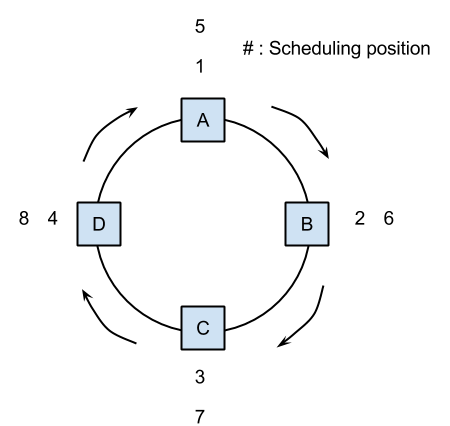
\includegraphics[width=0.5\textwidth]{./Images/round-robin.png}
\caption{Scheme of a round-robin scheduling}
\end{center}
\end{figure}}
\end{itemize}
 
\footnote{\url{https://github.com/Soulou/msc-thesis-container-balancer-controller}}

\subsection{Balancer client}

The balancer client, is a command line tool to command the controller, it
shows in a human-understandable way, the JSON results the controller and allows
a user to execute requests easily. Its documentation can be found in the
Appendix C: "~\nameref{app:client-doc}".

\footnote{\url{https://github.com/Soulou/msc-thesis-container-balancer-client}}

\subsection{Deployment}

All those services and tools have to be deployed on the instances of the
infrastructure.  More and more configuration managers (CM) are released those days to
answer the increasing needs to deploy applications in volatiles infrastructure,
composed of temporary virtual machines. To setup all the different pieces of
this infrastructure, \textbf{Ansible} has been used. There are two main models
of CMs, those centralized around a server, like \textbf{Chef Server} or \textbf{Puppet},
where the nodes synchronize themselves with this server. The devops do not connect
directly to the nodes but give instructions to the central server. The second
category are those who are run from a devops workstation, like \textbf{Chef Solo},
\textbf{Ansible}, \textbf{SaltStack}. The choice of \textbf{Ansible} has been done
for it's ability to deploy nodes in parallel and by it's easiness of prototyping,
its syntax is pretty simple.

All the mecanisms of deployment can be found on following \textit{GitHub} page:
\url{https://github.com/Soulou/msc-thesis-cloud-builder}. The script requires
that \textbf{Openstack} credentials are stored in environment variables. (
\texttt{OS\_USERNAME, OS\_TENANT\_NAME, OS\_PASSWORD, OS\_AUTH\_URL,
OS\_REGION\_NAME}). Then it uses the API to instantiates VMs, and then deploy
all the services on them using ansible \footnote{Ansible configuration:
\url{https://github.com/Soulou/msc-thesis-cloud-builder/tree/master/ansible}}.

